\begin{figure}
	\centering
	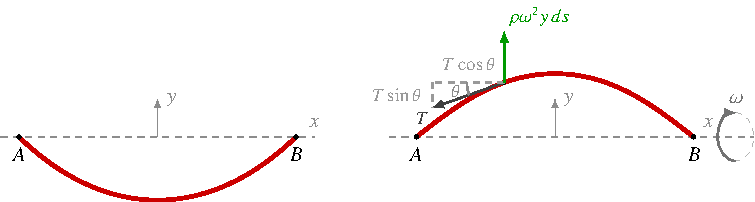
\includegraphics[width=\textwidth]{papers/elliptisch/images/troposkein.pdf}
	\caption{Links die hängende Schnur zwischen $A$ und $B$ bei
	$x = \pm l$, die Kettenlinie
	$y(x) = d\,(\cosh(x/d) - \cosh(l/d))$.
	Rechts rotierend um $AB$, das Troposkein
	\mbox{$y(x) = a\operatorname{sn}((x+l)/c, k)$}, mit
	Zentrifugalkraft $\rho\omega^2y\,ds$ und Seilspannung $T$ am
	Element mit Winkel $\theta$.}
	\label{fig:elliptisch:troposkein}
\end{figure}
